\section{Determining a simple DE from a description}

\subsection*{Resources}
\begin{itemize}
    \item Text: \url{http://tutorial.math.lamar.edu/Classes/DE/Definitions.aspx}
    \item Book: Chapter 1.2
\end{itemize}

\subsection*{Challenge}
Newton's law of cooling states that the rate of cooling of an object is proportional to the temperature difference with the ambient surroundings. (a) Write a differential equation describing this situation. (b) Assuming a proportionality constant of \num{0.2} \si{/hour}, what is the rate of temperature change when the object is at \SI{30}{\degreeCelsius} and the ambient temperature is \SI{20}{\degreeCelsius}?

\subsection*{Solution}
\six{\degreeCelsius/hour}

\hash{q}{078383}

\timebox



%%%%%%%%%%%%%%%%%%%%%%%%%%%%%%%%%
\newpage
%%%%%%%%%%%%%%%%%%%%%%%%%%%%%%%%%
\section{Direction (Slope) fields}

\subsection*{Resources}
\begin{itemize}
    \item Text: \url{http://tutorial.math.lamar.edu/Classes/DE/DirectionFields.aspx}
    \item Video 1: \url{https://www.khanacademy.org/math/differential-equations/first-order-differential-equations/differential-equations-intro/v/creating-a-slope-field}
    \item Video 2: \url{https://www.khanacademy.org/math/differential-equations/first-order-differential-equations/differential-equations-intro/v/slope-field-to-visualize-solutions}
    \item Book: Chapters 1.1, 1.2
\end{itemize}

\subsection*{Comment}
It is good practise to try drawing the below fields before looking at the next page. You need to be able to go in both directions (ie, drawing and recognising).

\subsection*{Question}
Try drawing the slope field for at least 3 of the equations given below (your choice). Then, put the slope fields given on the next page in the same order as these equations.

\begin{enumerate}
    \item $y'=x$
    \item $y'=0.2y$
    \item $y'=0.2y(1-y/6)$
    \item $y'=(x-y)/(x+y)$
    \item $y'=2(y-1)/x$
    \item $y'=2y/(x+5)$
\end{enumerate}

\newpage

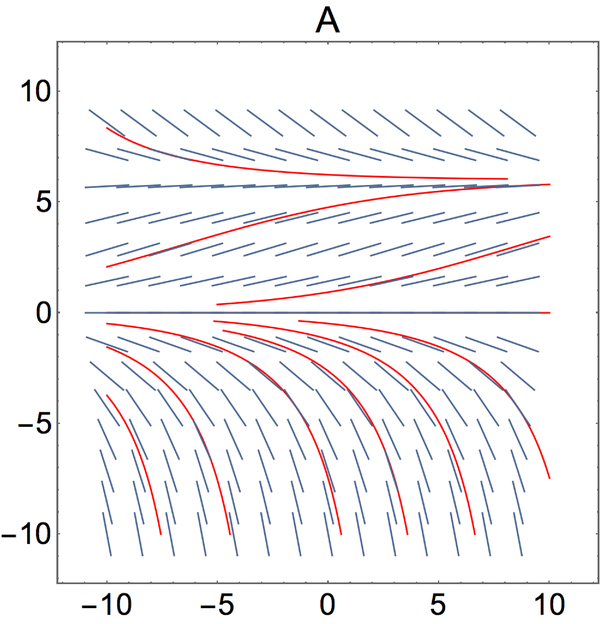
\includegraphics{direction_fields_A.png}
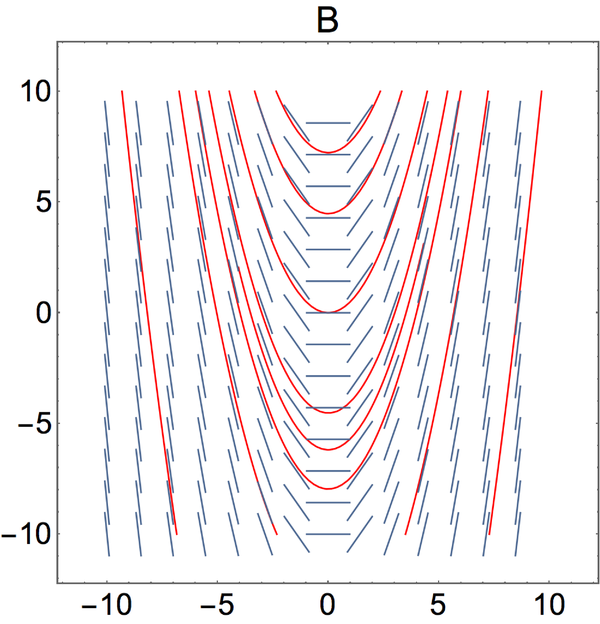
\includegraphics{direction_fields_B.png}
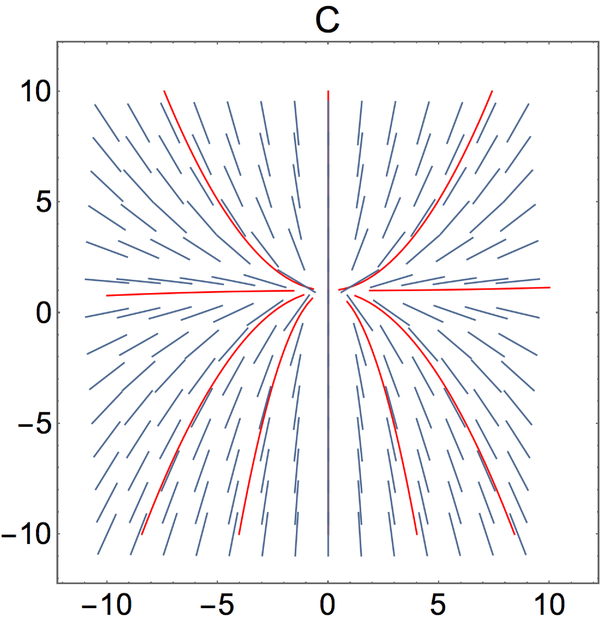
\includegraphics{direction_fields_C.png}

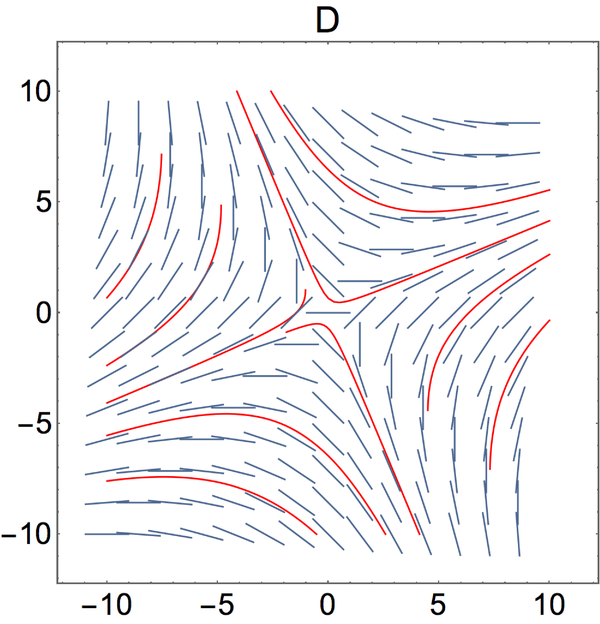
\includegraphics{direction_fields_D.png}
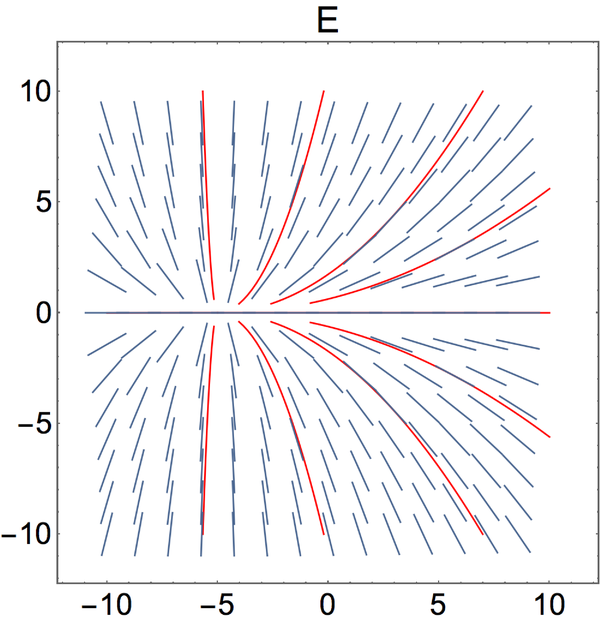
\includegraphics{direction_fields_E.png}
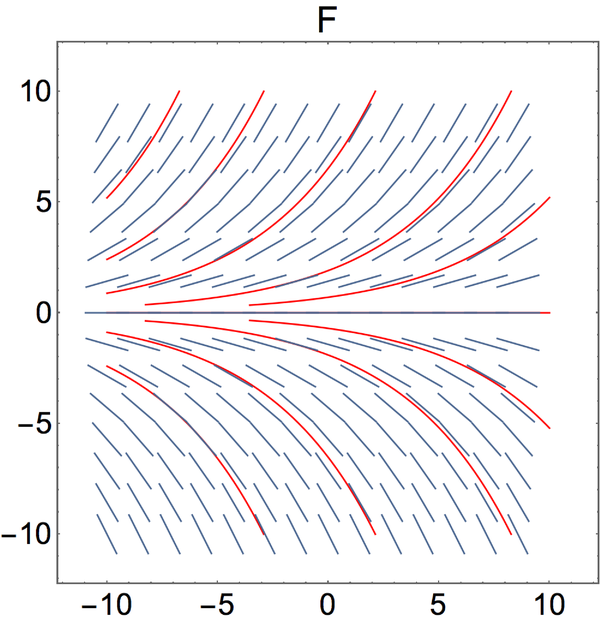
\includegraphics{direction_fields_F.png}

\subsection*{Solution}
\six{} (eg, ``abcdef'')

\hash{q}{743eb9}

\timebox


%%%%%%%%%%%%%%%%%%%%%%%%%%%%%%%%%
\newpage
%%%%%%%%%%%%%%%%%%%%%%%%%%%%%%%%%
\section{Solving a simple 1st-order linear equation}

\subsection*{Resources}
\begin{itemize}
    \item Video: \url{https://www.khanacademy.org/math/differential-equations/first-order-differential-equations/differential-equations-intro/v/finding-particular-linear-solution-to-differential-equation}
\end{itemize}

\subsection*{Comment}
It's not easy to see when equations can be solved simply, like in the challenge below, and when they can not. But for a 1st-order linear differential equation, this method is often good to try first. If it's not 1st order and not linear, you know to try a different approach.

\subsection*{Challenge}
Determine the value of $y(x=1)$ for the following equation:

\begin{equation}
    y'=2y-5x+2
\end{equation}

\subsection*{Solution}
\six{}

\hash{u}{505c7b}

\timebox



%%%%%%%%%%%%%%%%%%%%%%%%%%%%%%%%%
\newpage
%%%%%%%%%%%%%%%%%%%%%%%%%%%%%%%%%
\section{Separable equations I}

\subsection*{Resources}
\begin{itemize}
    \item Video I: \url{https://www.khanacademy.org/math/differential-equations/first-order-differential-equations/separable-equations/v/separable-differential-equations-introduction} 
    \item Video II: \url{https://www.khanacademy.org/math/differential-equations/first-order-differential-equations/separable-equations/v/particular-solution-to-differential-equation-example}
    \item Text:\url{http://tutorial.math.lamar.edu/Classes/DE/Separable.aspx}
\end{itemize}

\subsection*{Challenge}
Given the following equation:
\begin{equation}
    r' = -Sin(\theta)
\end{equation}
Determine the function $r(\theta)$ that passes through the point (0,1) in $\theta-r$ space, and then solve for $\theta = \pi/4$.


\subsection*{Solution}
\six{}

\hash{i}{286117}

\timebox



%%%%%%%%%%%%%%%%%%%%%%%%%%%%%%%%%
\newpage
%%%%%%%%%%%%%%%%%%%%%%%%%%%%%%%%%
\section{Separable equations II}

\subsection*{Resources}
\begin{itemize}
    \item Video I: \url{https://www.khanacademy.org/math/differential-equations/first-order-differential-equations/separable-equations/v/separable-differential-equations-introduction} 
    \item Video II: \url{https://www.khanacademy.org/math/differential-equations/first-order-differential-equations/separable-equations/v/particular-solution-to-differential-equation-example}
    \item Text:\url{http://tutorial.math.lamar.edu/Classes/DE/Separable.aspx}
\end{itemize}

\subsection*{Challenge}
Given the following equation:
\begin{equation}
    r' cot(\theta) + r = 2
\end{equation}
Determine the function $r(\theta)$ that passes through the point (0,1) in $\theta-r$ space, and then solve for $\theta = \pi/4$.

\subsection*{Solution}
\six{}

\hash{o}{87ee92}

\timebox



%%%%%%%%%%%%%%%%%%%%%%%%%%%%%%%%%
\newpage
%%%%%%%%%%%%%%%%%%%%%%%%%%%%%%%%%
\section{Separable equations III}

\subsection*{Resources}
\begin{itemize}
    \item Video I: \url{https://www.khanacademy.org/math/differential-equations/first-order-differential-equations/separable-equations/v/separable-differential-equations-introduction} 
    \item Video II: \url{https://www.khanacademy.org/math/differential-equations/first-order-differential-equations/separable-equations/v/particular-solution-to-differential-equation-example}
    \item Text:\url{http://tutorial.math.lamar.edu/Classes/DE/Separable.aspx}
\end{itemize}

\subsection*{Challenge}
Given the following equation:
\begin{equation}
    y' x^2 - y = 0
\end{equation}
Determine the function $y(x)$ that passes through the point $x=2,y=1$ and then solve for the given $x$ value. State the value of $x$ where the solution is undefined. % Would be nice to couple this with a field graph.

\subsection*{Solution}
Solve for $x=4$:

\six{}

\hash{p}{7cb08e} 

Value of x where solution is undefined:

\six{}

\hash{a}{b30fe7} 

\timebox




\stepcounter{section}




%%%%%%%%%%%%%%%%%%%%%%%%%%%%%%%%%
\newpage
%%%%%%%%%%%%%%%%%%%%%%%%%%%%%%%%%
\section{Logistic equation}

\subsection*{Resources}
\begin{itemize}
    \item Videos: The 5 videos on the logistic differential equation and function starting at: \url{https://www.khanacademy.org/math/differential-equations/first-order-differential-equations/logistic-differential-equation/v/modeling-population-with-differential-equations}
\end{itemize}

\subsection*{Comment}
The rate of growth can be calculated considering the equation $dN/dt=rN$. This was not clear in an earlier version of the challenge. The question has also been adjusted (100 mg instead of 300 mg) to minimise the chance of rounding errors effecting final answer. The hash-code has been updated to reflect this.

\subsection*{Challenge}
Assuming there is no-limit on growth, a given bacteria would be able to reproduce at such a rate that the amount of bacteria measured in mg increases by 20\% every 25 hours. However, due to environmental factors the limiting (maximum) amount of bacteria that can exist in the system at any one time is 400 mg. Assuming an initial amount of bacteria of 20 mg, how much time, rounded to the nearest integer hours, must one wait to reach 100 mg of bacteria?

\emph{Note: Be sure to maintain a sufficient number of significant figures in your numbers while performing the calculation.}

\subsection*{Solution}
\six{hours} (expressed as an integer - do not enter ``.00''.)

\hash{d}{0eba84} 

\timebox



%%%%%%%%%%%%%%%%%%%%%%%%%%%%%%%%%
\newpage
%%%%%%%%%%%%%%%%%%%%%%%%%%%%%%%%%
\section{Autonomous differential equations}

\subsection*{Resources}
\begin{itemize}
    \item Text: \url{http://tutorial.math.lamar.edu/Classes/DE/EquilibriumSolutions.aspx}
    \item Wikipedia: \url{https://en.wikipedia.org/wiki/Autonomous_system_(mathematics)}
\end{itemize}

\subsection*{Challenge}
Add the points of the autonomous differential equations in the following list:

1 point: $y' = cos(y)-5$

2 points: $y' = cos(y)/x - 5$

4 points: $y' = cos(y)/x - 5/x$

8 points: $y^2 = y' y+5$

16 points: $x y' = 5 y$

32 points: $y' = 1$

\subsection*{Solution}
\six{}

\hash{f}{9bf043} 
% Would be good to add some vector fields to show that it's independent of x.
\timebox




%%%%%%%%%%%%%%%%%%%%%%%%%%%%%%%%%
\newpage
%%%%%%%%%%%%%%%%%%%%%%%%%%%%%%%%%
\section{The stability of solutions I}

\subsection*{Resources}
\begin{itemize}
    \item Text: \url{http://tutorial.math.lamar.edu/Classes/DE/EquilibriumSolutions.aspx}
    \item Text: \url{http://www.math.psu.edu/tseng/class/Math251/Notes-1st\%20order\%20ODE\%20pt2.pdf}
\end{itemize}

\subsection*{Challenge}
Considering the logistic equation $N'=0.2N(1-N/6)$, make 3 separate lists containing any equilibrium, semi-stable and unstable y-values.

To check your answer, sum the value of each list. If there are no values in a list, simply enter ``none'' to check the result.

\subsection*{Solution}
\subsubsection*{Stable}
\six{}

\hash{g}{2c32d8} 

\subsubsection*{Semi-stable}
\six{}

\hash{h}{8b595d} 

\subsubsection*{Unstable}
\six{}

\hash{j}{4fd3f6}

\timebox



%%%%%%%%%%%%%%%%%%%%%%%%%%%%%%%%%
\newpage
%%%%%%%%%%%%%%%%%%%%%%%%%%%%%%%%%
\section{The stability of solutions II}

\subsection*{Resources}
\begin{itemize}
    \item Text: \url{http://tutorial.math.lamar.edu/Classes/DE/EquilibriumSolutions.aspx}
    \item Text: \url{http://www.math.psu.edu/tseng/class/Math251/Notes-1st\%20order\%20ODE\%20pt2.pdf}
\end{itemize}

\subsection*{Challenge}
Considering the differential equation $y'=(y^2-16)(y+3)^2$, make 3 separate lists containing any equilibrium, semi-stable and unstable y-values.

To check your answer, sum the value of each list. If there are no values in a list, simply enter ``none'' to check the result.

\subsection*{Solution}
\subsubsection*{Stable}
\six{}

\hash{k}{667798} 

\subsubsection*{Semi-stable}
\six{}

\hash{z}{200aa3} 

\subsubsection*{Unstable}
\six{}

\hash{x}{d1ee5b}

\timebox



%%%%%%%%%%%%%%%%%%%%%%%%%%%%%%%%%
\newpage
%%%%%%%%%%%%%%%%%%%%%%%%%%%%%%%%%
\section{Euler's method}

\subsection*{Resources}
\begin{itemize}
    \item Videos and exersizes in the ``Euler's Method'' section of Khan academy: \url{https://www.khanacademy.org/math/differential-equations/first-order-differential-equations/eulers-method-tutorial/v/eulers-method}
    \item Text: \url{http://tutorial.math.lamar.edu/Classes/DE/EulersMethod.aspx}
\end{itemize}

\subsection*{Challenge}
Considering the differential equation $y'=10-y$, an initial value of $y(0)=1$ and a step size of $\Delta x = 0.2$, use Euler's method to estimate the value of $y(x=1)$. The actual solution, $y(x)=10-9e^{-x}$, is shown below.

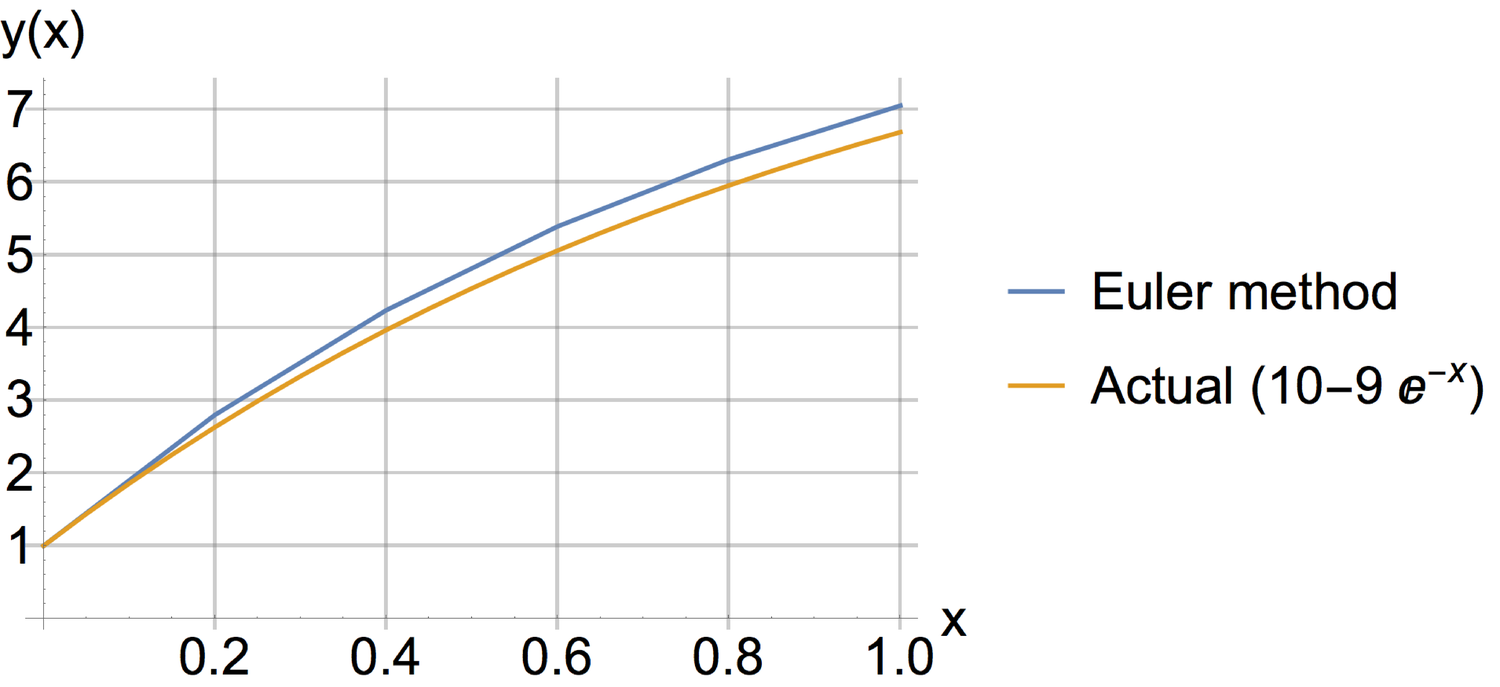
\includegraphics{eulers_method.png}

\subsection*{Solution}
\six{}

\hash{c}{1f90fa} 
% It would be nice to see if this error actually goes to zero in the end.
\timebox




%%%%%%%%%%%%%%%%%%%%%%%%%%%%%%%%%
\newpage
%%%%%%%%%%%%%%%%%%%%%%%%%%%%%%%%%
\section{Exact differential equations: derivation}

\subsection*{Resources}
\begin{itemize}
    \item Videos: \url{https://www.khanacademy.org/math/differential-equations/first-order-differential-equations/exact-equations/v/exact-equations-intuition-1-proofy}
\end{itemize}

\subsection*{Challenge}
Please follow the two videos on derivation and intuition regarding exact differential equations starting at the video listed above.

If
\begin{equation}
    \frac{d \psi(x,y)}{dx} = 2xy + x^2y' - (x+y)/100
\end{equation}

what is $\displaystyle \frac{\partial \psi}{\partial x}$?

To check your answer, substitute $x=3.1$ and $y=-2$ into the resulting equation.

\subsection*{Solution}
\six{}

\hash{v}{f7f178}
% Note that video is not so clear about psi being a full rather than partial derivative. This question should help address this problem.
\timebox




%%%%%%%%%%%%%%%%%%%%%%%%%%%%%%%%%
\newpage
%%%%%%%%%%%%%%%%%%%%%%%%%%%%%%%%%
\section{Exact differential equations: possible solutions given $\psi_x$}

\subsection*{Resources}
\begin{itemize}
    \item Videos: Exact equations intuition 1,2 and examples 1,2,3 starting from \url{https://www.khanacademy.org/math/differential-equations/first-order-differential-equations/exact-equations/v/exact-equations-intuition-1-proofy}
    \item Text: \url{http://tutorial.math.lamar.edu/Classes/DE/Exact.aspx}
\end{itemize}

\subsection*{Challenge}
Sum the points of all the possible solutions to the integral of the partial-differential equation:
\begin{equation}
    \psi_x = 6x - 3e^x sin(y)
\end{equation}

1 point: $\psi(x,y) = 3x^2-3e^x sin(y) + 4$

2 points: $\psi(x,y) = 3x^2-3e^x sin(y) + x$

4 points: $\psi(x,y) = 3x^2-3e^x sin(y) + y$

8 points: $\psi(x,y) = 3x^2-3e^x sin(y) + yx$

16 points: $\psi(x,y) = 3x^2-3e^x sin(y) + y^2$

32 points: $\psi(x,y) = 3x^2-3e^x sin(y) + 5 sin(y)$

64 points: $\psi(x,y) = 3x^2-3e^x sin(y) + 5 sin(y)cos(x)$

\subsection*{Solution}
\six{}

\hash{b}{408993} 

\timebox



%%%%%%%%%%%%%%%%%%%%%%%%%%%%%%%%%
\newpage
%%%%%%%%%%%%%%%%%%%%%%%%%%%%%%%%%
\section{Exact differential equations: identification}
\label{sec:edeid}

\subsection*{Resources}
\begin{itemize}
    \item Videos: Exact equations intuition 1,2 starting from \url{https://www.khanacademy.org/math/differential-equations/first-order-differential-equations/exact-equations/v/exact-equations-intuition-1-proofy}
    \item Text: \url{http://tutorial.math.lamar.edu/Classes/DE/Exact.aspx}
\end{itemize}

\subsection*{Challenge}
Sum the points of the equations below that are exact differential equations:

1 point: $\displaystyle (3x^2y+8xy^2) dx + (x^3 + 8x^2y + 12 y^2) dy = 0$ % A

2 points: $\displaystyle sin(x) cos(y) dx + cos(x) sin(y) dy = 0$ % B

4 points: $\displaystyle sin(x) cos(y) dx + sin(x) sin(y) dy = 0$ % C

8 points: $\displaystyle \frac{dx}{x} + \frac{dy}{y} = 0$ % D

16 points: $\displaystyle -\frac{y dx + x dy}{x^2} = 0 $ % E

32 points: $\displaystyle -\frac{y dx - x dy}{x^2} = 0$ % F


\subsection*{Solution}
\six{}

\hash{n}{868f48} 

\timebox



%%%%%%%%%%%%%%%%%%%%%%%%%%%%%%%%%
\newpage
%%%%%%%%%%%%%%%%%%%%%%%%%%%%%%%%%
\section{Exact differential equations: solving}

\subsection*{Resources}
\begin{itemize}
    \item Videos: Exact equations examples 1,2,3 starting from \url{https://www.khanacademy.org/math/differential-equations/first-order-differential-equations/exact-equations/v/exact-equations-example-1}
    \item Text: \url{http://tutorial.math.lamar.edu/Classes/DE/Exact.aspx}
\end{itemize}

\subsection*{Challenge}
In challenge \ref{sec:edeid} you should have identified 4 exact differential equations. Considering each of the 4 EDE's in order, try to solve the EDE's applying the following conditions:

\subsubsection{1st EDE}
Do not try to solve this one.

\subsubsection{2nd EDE}
Use the condition $y(\pi/4)=\pi/4$ to find an explicit solution for the equation and then evaluate $y$ at $x=\pi$.

\subsubsection{3rd EDE}
Use the condition $y(1)=3$ to find an explicit solution for the equation and then evaluate $y$ at $x=4$.

\subsubsection{4th EDE}
Use the condition $y(1)=2$ to find an explicit solution for the equation and then evaluate $y$ at $x=1$.


\subsection*{Solution}

\subsubsection{2nd EDE}
\six{}

\hash{m}{af87e2}

\subsubsection{3rd EDE}
\six{}

\hash{aa}{d01c3d}

\subsubsection{4th EDE}
\six{}

\hash{bb}{5e1074}

\timebox




%%%%%%%%%%%%%%%%%%%%%%%%%%%%%%%%%
\newpage
%%%%%%%%%%%%%%%%%%%%%%%%%%%%%%%%%
\section{Exact differential equations: a useful integration method}

\subsection*{Challenge}
Obtain an expression for $g(x)$ in terms of $f(x)$ in the following integral:

\begin{equation}
    \int \frac{f'(x)}{f(x)} dx = g(x)
\end{equation}

ie, you should be able to re-write $g(x)$ in terms of a simple (non-integral) function of $f(x)$, in the form $g(x) = \cdots$.

\subsection*{Solution}
You can check your answer by putting a function of $x$ into $f(x)$.

\timebox




%%%%%%%%%%%%%%%%%%%%%%%%%%%%%%%%%
\newpage
%%%%%%%%%%%%%%%%%%%%%%%%%%%%%%%%%
\section{Exact differential equations: integrating factors}
\label{sec:edeif}

\subsection*{Resources}
\begin{itemize}
    \item Videos: Integrating factors 1,2 starting from \url{https://www.khanacademy.org/math/differential-equations/first-order-differential-equations/exact-equations/v/integrating-factors-1}
\end{itemize}

\section*{Comment}
Note that in the videos, Sal Khan does an example considering an integrating factor of $\mu(x)$, but in some cases $\mu(y)$ leads to a solution more easily. You may need to try both to determine an answer.

\subsection*{Challenge}
Solve the exact differential equations below using integrating factors.

1. Solve the equation below using an integrating factor. Place the solution in the form $f(x,y) = C$, then calculate the value of $C$ when substituting $x=2$ and $y=1$ into the equation. Do not try to solve the equation to get it in the form $y(x)=\cdots$.

\begin{equation}
    \label{eq:edeif1}
    y dx + (2 x y - e^{-2 y}) dy = 0
\end{equation}

2. Calculate the integrating factor for the following equation. To check your answer, substitute $x=1$ or $y=1$ into any final expression, assuming an integration constant of zero.

\begin{equation}
    \label{eq:edeif2}
    y(3x-y) dx + x(x-y)dy = 0
\end{equation}

3. Show that $1/(x^y+y^2)$ is an integrating factor for the equation
\begin{equation}
    x dx + y dy + 4 y^3 (x^2 + y^2)dy = 0
\end{equation}

\subsection*{Solution}
Challenge related to equation \ref{eq:edeif1}: \hash{cc}{bb15d6}

Challenge related to equation \ref{eq:edeif2}: \hash{dd}{6a8742}

\timebox




%%%%%%%%%%%%%%%%%%%%%%%%%%%%%%%%%
\newpage
%%%%%%%%%%%%%%%%%%%%%%%%%%%%%%%%%
\section{Exact differential equations: integrating factor derivation}
\label{sec:intfacderiv}

\subsection*{Challenge}
1. Starting from the equation

\begin{equation}
    \mu(x,y) M(x,y) dx + \mu(x,y) N(x,y) dy = 0
\end{equation}

show that if the integrating factor $\mu$ is only a function of $x$, then

\begin{equation}
    \label{eq:intfacmux}
    \mu_x = \mu \left ( \frac{M_y-N_x}{N} \right )
\end{equation}

2. Do the same, assuming that $\mu$ is only a function of $y$.

% NT do something for linear equations mu=e^\int(a)

\timebox




%%%%%%%%%%%%%%%%%%%%%%%%%%%%%%%%%
\newpage
%%%%%%%%%%%%%%%%%%%%%%%%%%%%%%%%%
\section{Exact differential equations: integrating factor calculation}
\label{sec:edeifcalc}

\section*{Comment}
Without proof, we can use equation \ref{eq:intfacmux} to gain information about the existance of an integration factor. If $\left ( \frac{M_y-N_x}{N} \right )$ is a function of $x$ only, then we know that the integration factor is only a function of $x$, and it can be solved for by integration of equation \ref{eq:intfacmux}. The same can be said for $\mu(y)$ that you derived an expression for in challenge \ref{sec:intfacderiv}.

\subsection*{Challenge}
Use equations from section \ref{sec:intfacderiv} and information provided in the comment here to determine the integrating factor for

\begin{equation}
    \label{eq:edeifcalc1}
    e^x dx + (e^x Cot(y) + 2y Csc(y)) dy = 0
\end{equation}

and

\begin{equation}
    \label{eq:edeifcalc2}
    (x-y^2) dx + 2xy dy = 0
\end{equation}

To check your answer, for both cases substitute $x=\pi$ or $y=\pi$ into the integrating factor, and assume an integration constant of 1.

\subsection*{Solution}


Equation \ref{eq:edeifcalc1}: \hash{ee}{51a0ae}

Equation \ref{eq:edeifcalc2}: \hash{ff}{a56bce}


\timebox




%%%%%%%%%%%%%%%%%%%%%%%%%%%%%%%%%
\newpage
%%%%%%%%%%%%%%%%%%%%%%%%%%%%%%%%%
\section{Summary of 1st-order differential equations}

\subsection*{Challenge}
1. Create a flowchart describing how you will approach solving a general 1st-order differential equation.

% Linear, Separable, Exact (with and without integration factors)
2. Solve the following 1st-order differential equations:

\begin{equation}
    \label{eq:1odegen1}
    y' - 4y = 8x + 3
\end{equation}
evaluated at $x=1$.

\begin{equation}
    \label{eq:1odegen2}
    4yy' = 8x + 3
\end{equation}
assuming an integration constant of zero and evaluating the final equation at $x=2$.

\begin{equation}
    \label{eq:1odegen3}
    y' + 4y = e^{-8x}
\end{equation}
assuming an integration constant of zero and evaluating the final equation at $x=1/8$.

\subsection*{Solution}
Equation \ref{eq:1odegen1}: \hash{qq}{a43ab2}

Equation \ref{eq:1odegen2}: \hash{rr}{990bfa}

Equation \ref{eq:1odegen3}: \hash{ss}{91989d}

\timebox



% Remaining Khan 1st-order equations
% Benouli and substitution

% About 4.5 weeks on 1st-order and 4.5 weeks on 2nd order?
% Khan covers 1st-order well but 2nd-order not so much.
% Follow Khan for 1st-order, then do 2nd order and fill in holes with Paul's notes - this may cause issues if terminology is different.
% More advanced topics are in Paul's notes, but first check how much time is remaining.

% Do I need to add more challenges for simple 1st order linear equations?
